\documentclass{standalone}
\usepackage{tikz}
\usetikzlibrary{shadows, arrows}

\renewcommand{\familydefault}{\sfdefault}

\definecolor{lightBlue}{RGB}{46, 172, 228}
\definecolor{darkBlue}{RGB}{30, 65, 81}

\tikzset{
    shade border north to south/.style args={#1 to #2}{
        postaction={draw, very thick, path fading=south, #1},
        postaction={draw, very thick, path fading=north, #2}
    }
}

\begin{document}
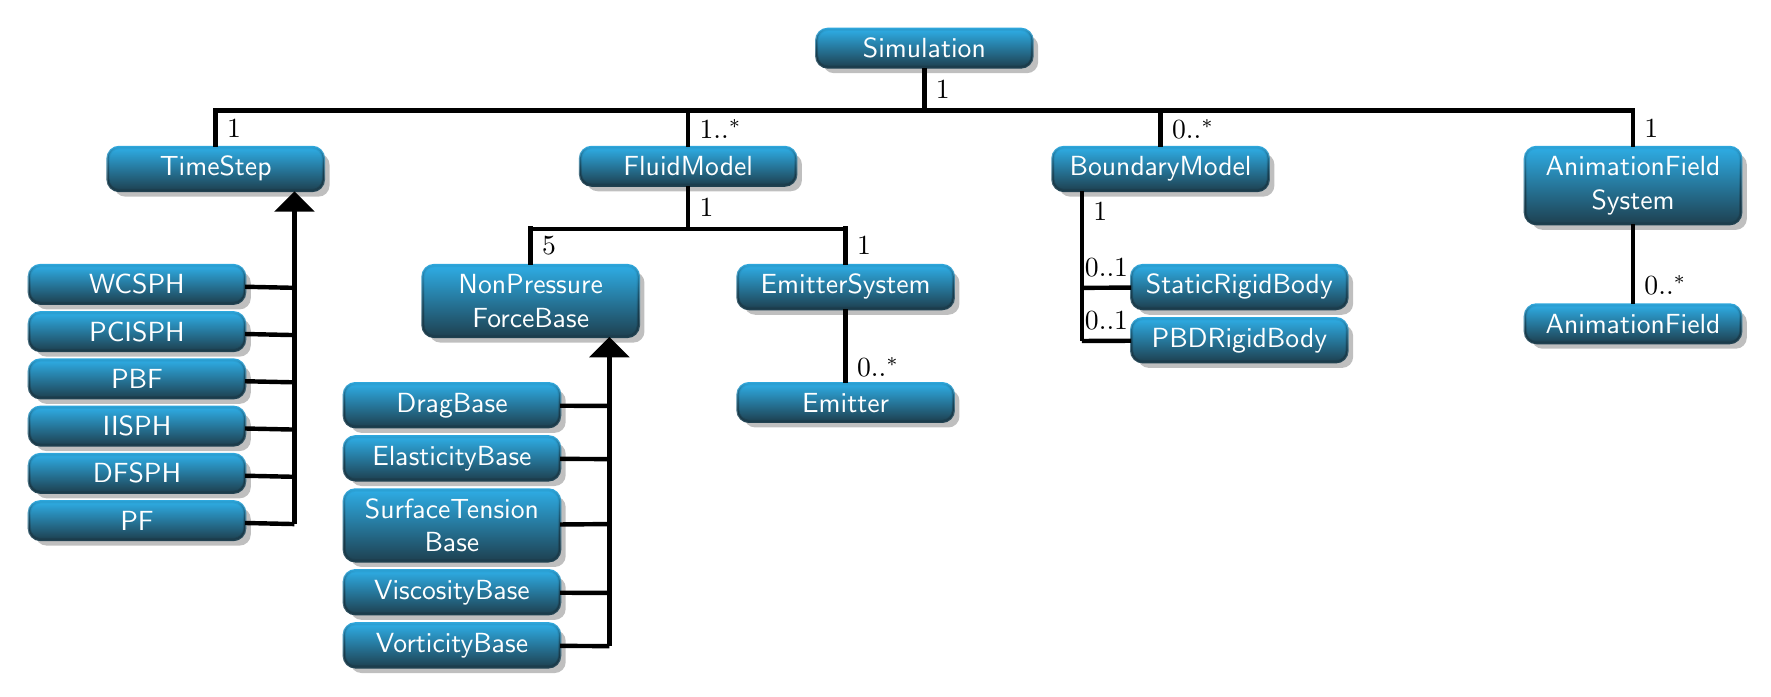
\begin{tikzpicture}[
	class/.style={
		rounded corners, rectangle, draw, align=center, top color=lightBlue,
		bottom color=darkBlue, text=white, drop shadow, shade, shade border
		north to south=lightBlue!97!black to darkBlue!97!black, text width=2.5cm, anchor=mid
	}
]
\node[class] (Sim) at (0,0) {Simulation};

% Time Step
\node[class] (Time) at (-9, -1.5) {TimeStep};
	% Pressure Solvers
	\foreach \x/\y in {WCSPH/0, PCISPH/1, PBF/2, IISPH/3, DFSPH/4, PF/5} {
		\node[class] (\x) at (-10, -3 - \y*0.6) {\x};
		\draw[ultra thick] (-8, -2.4 - \y*0.6) -- (-8, -3 - \y*0.6); 
		\draw[ultra thick] (-8, -3 -\y*0.6) -- (\x);
	}

% Fluid Models
\node[class] (Fluid) at (-3, -1.5) {FluidModel};
	% Non Pressure Force Base Class
	\node[class] (NonPressure) at (-5, -3) {NonPressure ForceBase};
		%Non Pressure Forces Implementation
		\foreach \x/\y in {DragBase/-4.5, ElasticityBase/-5.175, ViscosityBase/-6.875, VorticityBase/-7.55} {
			\node[class] (\x) at (-6, \y) {\x};
			\draw[ultra thick] (\x) -- (-4, \y);
		}
		\node[class] (SurfaceTension Base) at (-6, -5.85) {SurfaceTension Base};
		\draw[ultra thick] (SurfaceTension Base) -- (-4, -6);
% Emitters
\node[class] (Emitter) at (-1, -3) {EmitterSystem};
	% Emitter Implementation
	\node[class] (Emit) at (-1, -4.5) {Emitter};

% Boundaries
\node[class] (Boundary) at (3, -1.5) {BoundaryModel};
	% Boundary classes
	\node[class] (Static) at (4, -3) {StaticRigidBody};
	\node[class] (Dynamic) at (4, -3.675) {PBDRigidBody};

% AnimationFieldSystem
\node[class] (AnimField) at (9, -1.5) {AnimationField System};
	% Animation Fields
	\node[class] (Anim) at (9, -3.5) {AnimationField};

% Lines
\draw[ultra thick] (Sim) -- node[right] {$1$} (0, -.75);

\draw[ultra thick] (0, -.75) -- (-9, -.75) -- node[right] {$1$} (Time);
\draw[ultra thick] (-3, -.75) -- node[right] {$1..^*$} (Fluid);
\draw[ultra thick] (0, -.75) -- (3, -.75) -- node[right] {$0..^*$} (Boundary);
\draw[ultra thick] (3, -.75) -- (9, -.75) -- node[right] {$1$} (AnimField);

\draw[{triangle 90}-, ultra thick] (-8,-1.775) -- (-8, -3);

\draw[ultra thick] (Fluid) -- node[right] {$1$} (-3, -2.25);
\draw[ultra thick] (-3, -2.25) -- (-5, -2.25);
\draw[ultra thick] (-5, -2.22) -- node[right] {$5$} (NonPressure);
\draw[ultra thick] (-3, -2.25) -- (-1, -2.25);
\draw[ultra thick] (-1, -2.22) -- node[right] {$1$} (Emitter);

\draw[{triangle 90}-, ultra thick] (-4, -3.625) -- (-4, -7.55);

\draw[ultra thick] (Emitter) -- node[right, yshift=-.75em] {$0..^*$} (Emit);

\draw[ultra thick] (2, -1.775) -- node[right, yshift=1em] {$1$} (2, -3) -- (2, -3.675);
\draw[ultra thick] (2, -3) -- node[above] {$0..1$} (Static);
\draw[ultra thick] (2, -3.675) -- node[above] {$0..1$} (Dynamic);

\draw[ultra thick] (AnimField) -- node[right, yshift=-.75em] {$0..^*$} (Anim);
\end{tikzpicture}
\end{document}